\chapter{走进IT项目管理}
\section{项目与项目管理的价值}
\subsection{项目的价值}
项目是实现价值、成就事业的载体。
\begin{itemize}
	\item 通过日常工作来维持基本地运行;
	\item 通过项目来推进自身地发展和壮大。
\end{itemize}
\subsection{项目管理的价值}
\begin{enumerate}
	\item 项目管理无处不在、无时不在,项目管理既是项目成功的要素,也是项目失败的根源;
	\item 项目的价值来源于项目目标的完成,有效管理可以创造更大价值;
	\item 许多跨国公司经验,企业的成功在于有效地推行项目管理;
	\item 项目管理是一种有效地知识积累方式,也是进行知识管理的有效途径;
	\item 越来越多的企业引入项目管理,把它作为主要的运作模式和提高企业运作效率的解决方案。
\end{enumerate}
\section{走进项目}
项目已成为推动人类生产与进步的主要动力;
\subsection{人类活动特点}
\begin{itemize}
	\item 目的性:为了达到预期的目的而活动;
	\item 依存性:分工越来越细,依存越来越紧密;
	\item 知识性:在实践与经验中学习,形成知识体系。
\end{itemize}
\subsection{作业与项目}
活动分化为两类:
\begin{itemize}
	\item 作业(Operations):连续不断、周而复始的活动,如车间加工产品的活动、财务人员的日常记账工作等。
	\item 项目(Projects):临时性的、一次性的活动,如企业新产品开发、企业业务系统开发等。
\end{itemize}
\par 项目和作业的区别:
\begin{table}[!h]
	\begin{tabular}{|l|l|l|l|}
		\hline
		项目&作业&项目&作业\\
		\hline
		独一无二&重复的&多变的资源需求&稳定的资源需求\\
		\hline
		有限时间&无限时间&柔性的组织&稳定的组织\\
		\hline
		革命性的改变&渐进性的改变&效果性&效率性\\
		\hline
		状态的不平衡&平衡&风险和不确定性&经验性\\
		\hline
		目标之间不均衡&均衡&以达到目标为宗旨&以完成任务为宗旨\\
		\hline
	\end{tabular}
\end{table}
\subsection{项目的定义}
\noindent \textbf{国际项目管理协会}(International Project Management Association ,IPMA) 对项目的定义为:项目是一个特殊的、将被完成的有限任务,它是在一定时间内,满足一系列特定目标的多项相关工作的总称。\\
\textbf{英国项目管理协会}(Association for Project Management,APM)对项目的定义为:项目是由一系列具有开始和结束日期、相互协调和控制的活动组成的,通过实施而达到满足时间、费用和资源等约束条件的独特的过程。\\
\textbf{美国项目管理协会}(Project Management Institution,PMI)对项目的定义为:项目是为提供某项独特的产品、服务或成果所做的临时性努力。\\
\textbf{中国项目管理研究委员会}(Project Management Research Committee,PMRC)对项目的定义为:项目是一个特殊的将被完成的任务,它是在一定时间内,满足一系列特定目标的多项相关工作的总称。\\
\textbf{项目定义:}项目是为完成某一\textbf{独特的}产品和服务所做的\textbf{一次性}努力。
\subsection{项目的特征}
\begin{itemize}
	\item 独特性:范围、时间、成本、质量目标
	\item 一次性:不存在完全相同的项目
	\item 整体性:不是一项项孤立活动的堆积
	\item 临时性:有规定的时间段
	\item 不确定性:目标的复杂性和可变性
	\item 多变性:资源需求动态、多变、不确定
	\item 主要发起人:提供资金
\end{itemize}
\section{走进项目管理}
\subsection{管理的概念}
\par \textbf{管理:}管理是社会组织中,为了实现预期目标,以人为中心进行的协调活动。
\begin{enumerate}
	\item 目的:实现预期目标;
	\item 本质:协调;
	\item 产生于:社会组织;
	\item 中心:人;
	\item 方法:多种多样性。
\end{enumerate}
有效的管理者 = 理论掌握+技巧运用+思想化
\subsection{项目管理的定义}
项目管理:
\begin{itemize}
	\item \textbf{一种管理活动},即一种有意识地按照项目的特点和规律,对项目进行组织管理的活动;
	\item \textbf{一种管理学科},即以项目管理活动为研究对象的一门学科,它是探求项目活动科学组织管理的理论与方法。
\end{itemize}
PMI的定义:项目管理就是把各种知识、技能、手段和技术应用于项目活动之中,以达到项目的要求。项目管理是通过应用和综合诸如启动、规划、实施、监控和收尾等项目管理过程来进行的。项目经理是负责实现项目目标的个人。\\
PMRC的定义:项目管理就是以项目为对象的系统管理方法。通过一个临时性的专门的柔性组织,对项目进行高效率的计划、组织、指导和控制,以实现项目全过程的动态管理和项目目标的综合协调与优化。
\subsection{项目管理的特点}
\begin{itemize}
	\item 五项任务:项目计划、项目组织、质量管理、费用控制、进度控制;
	\item 注重综合性;
	\item 在\textbf{确定的期限}内生产出\textbf{不完全确定的}产品或完成\textbf{不完全确定的}任务;
\end{itemize}
另外还有特点:
\begin{itemize}
	\item 对象:项目或被当作项目来处理的运作;
	\item 全过程都贯穿着系统工程的思想;
	\item 组织具有特殊性;
	\item 体制是一种基于团队管理的个人;
	\item 方式是目标管理;
	\item 要点是创造和保持一种使项目能顺利进行的环境;
	\item 方法和手段具有先进性、开放性。
\end{itemize}
\subsection{项目管理知识体系}
两大项目管理研究体系,即以PMI 为代表的项目管理知识体系和IPMA 为代表的项目管理知识体系。
\subsubsection*{PMI\&PMBOK}
见下图
\begin{figure}[!h]
	\centering
	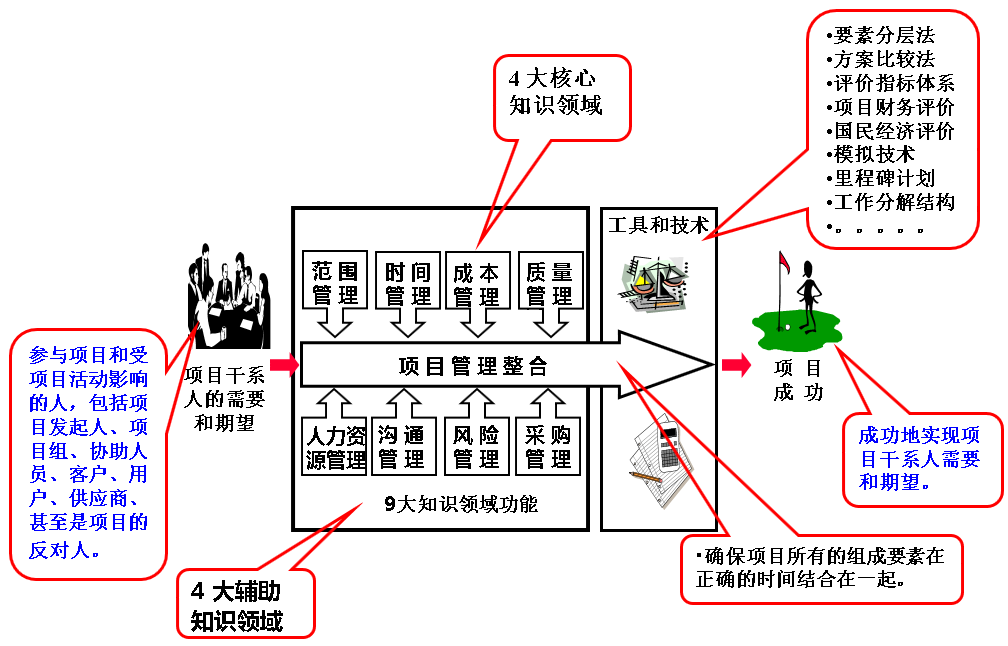
\includegraphics[width=0.8\textwidth]{image/1-1}
	\caption{基于PMBOK的项目管理框架}
\end{figure}
\subsubsection*{IPMA\&ICB}
PMRC于2001年推出了一个具有中国特色的项目管理知识体系(Chinese Project Management Body of Knowledge,C-PMBOK)。

\section{走进IT项目}
两大趋势:经济全球化和全球信息化。
\par 三大资源:材料、能源和信息。
\subsection{信息技术}
\par \textbf{信息技术}
(Information Technology,IT)是在信息科学的基本原理和方法的指导下扩展人类处理信息能力的技术,是以电子计算机和现代通信为主要手段,实现信息的获取、加工、传递和利用等功能的技术总和。
\par 信息技术:传感技术、通信技术、计算机技术和控制技术等。
\subsection{信息与信息化}
信息技术以信息为对象,以信息化为手段,以推动社会进步为目的。 
\subsubsection*{信息的概念}
信息是有价值的数据集合。
\begin{itemize}
	\item 信息是有一定含义的数据,是人们用来描述客观世界的知识;
	\item 信息是加工处理后的数据,是事物存在或运行状态的表达;
	\item 信息是对决策或行为有现实或潜在价值的数据。
\end{itemize}
\subsubsection*{信息的属性}
信息的属性:事实性、等级性、价值性、传输性、时效性、时间性、转换性。
\subsubsection*{信息化的概念}
信息化是指在经济、科技、社会各领域,在开发、生产、服务、管理、生活各层次,有效开发利用信息资源,建立先进的信息基础设施,发展信息技术及产业,加快国民经济发展和社会进步,提高综合国力和竞争力,提高生活、工作水平及质量。
\subsection{IT项目的概念}
\subsubsection*{IT项目的定义}
IT项目:利用有限资源、在一定的时间内,完成满足一系列特定的IT信息化目标的多项相关工作。
\subsubsection*{IT项目的分类}
\begin{itemize}
	\item 按产业属性划分
	\item 按物理形态划分
	\item 按用途划分
	\item 按范围划分
	\item 按使用对象划分
\end{itemize}
\subsubsection*{IT项目的特征}
IT项目具有特征:独特性、一次性、整体性、临时性、不确定性、资源多变性、有一个主要发起人等特征,还具有:
\begin{enumerate}
	\item 目标的不确定性
	\item 需求的不稳定性
	\item 费用的不可控性
	\item 项目的时限性
 	\item 对智力的依赖性
	\item 项目评价的主观性
	\item 项目的创新性
\end{enumerate}
\par IT项目的实施与管理,决不是一个简单的信息设备的购置和使用问题,而是建立新的价值观念、知识结构和心理态度的系统工程。
\section{走进IT项目管理}
\subsection{IT项目管理的定义}
\begin{itemize}
	\item 把各种知识、技能、手段和技术应用于IT项目活动之中,以达到IT项目的要求;
	\item 通过应用和综合诸如启动、规划、实施、监控和收尾等IT项目管理过程来进行的;
	\item 项目经理是负责实现IT项目目标的个人。
\end{itemize}
\subsection{IT项目管理的特点}
特点:与战略目标的相关性、与业务规则的一致性、环境基础的重要性、管理的集成性、人力资源管理的特殊性、项目过程的可控性、文档的完整性。
\subsection{IT项目管理知识体系}
三维结构模型:
\begin{itemize}
	\item 面向项目管理职能的职能型iPMBOK
	\item 面向项目管理过程的流程型iPMBOK
	\item 面向项目管理对象的离散型iPMBOK
\end{itemize}
\section{走进软件与软件项目}
\subsection{软件的定义}
软件(software)是计算机系统中与硬件(hardware)相互依存的另一部分,它是程序(program)、数据(data)和文档(document)的完整集合。
\subsection{软件的分类}
分类:软件功能划分、软件工作方式划分、软件规模划分、软件使用频度划分、软件失效的影响划分、软件服务对象划分、软件的有偿性和无偿性划分。
\subsection{软件的特点}
\begin{itemize}
	\item 软件产品的抽象性
	\item 软件生产过程的特殊性
	\item 软件缺陷检测的困难性
	\item 软件维护的复杂性
	\item 软件对环境的依赖性
	\item 软件开发方式与软件发展的不对称性
	\item 系统开销的主导性
	\item 与社会因素的关联性
\end{itemize}
\subsection{软件项目的分类与特点}
\subsubsection*{软件项目的定义}
软件项目:利用有限资源、在一定的时间内,完成满足一系列以软件为核心的多项相关工作。
\subsubsection*{软件项目的分类}
分类:软件功能划分、软件工作方式划分、软件规模划分、软件服务对象划分、软件的有偿性和无偿性。
\subsubsection*{软件项目的特点}
区别其他产品的最大区别是无形和没有物理属性。
\begin{enumerate}
	\item 高度复杂性
	\item 智力密集、可见性差
	\item 单件生产、过程不规范
	\item 劳动密集、自动化程度低
	\item 开发工作渗透了人的因素
	\item 开发方法多样性
\end{enumerate}
\section{走进软件项目管理}
\subsection{软件项目管理的意义}
\begin{itemize}
	\item 为了使软件项目能够按照预定的范围、成本、进度、质量顺利完成,而对范围、费用、时间、质量、人力资源、风险、采购等进行分析和管理的活动;
	\item 为了完成项目既定目标,需要通过软件项目管理过程来对软件任务进行组织、计划、实施、管理和评估,以明确和满足范围、时间、成本、质量等方面的约束限制。
\end{itemize}